
\section{Evaluation}
\begin{frame}
	
	\frametitle{ Evaluation of Proposed Approach }
	\framesubtitle{Performance Measures}

		\begin{itemize}
			\item<1->  $\mathit{Precision} =$ $ \mathit{\frac{\#\ of\ correct\ predictions}{\#\ of\ total\ predictions}}$ is the fraction of the produced predictions that are correct (i.e., a full match occurred within the prediction interval).   
			
			\item<2-> $\mathit{Spread} =end(I) -start(I)$ is the width of the prediction interval $I$.  
			
				\item<3->  $\mathit{Cumulative\ communication}$:
		   number of messages, which are required to perform the distributed online learning modes to synchronize the prediction models.
		\end{itemize}

\end{frame}



%\begin{frame}
%	
%	\frametitle{Initial Experimental Results }
%	\framesubtitle{Setup}
%1	analytical \& theoretical analysis 
% 2 evaluation with synthetic datastest \& 3 real datasets and grouping thing  
% then initial results 
%	
%\end{frame}


\begin{frame}
	
	\frametitle{Empirical evaluation }
	\framesubtitle{Experimental Setup}
\begin{itemize}
	\item<1-> Synopses over raw AIS messages in Brest, France: 1 October 2015 to 31 March 2016 (ais\_brest\_synopses.json). 
	
	\item<1->$ 4,684,444$ derived critical points.
	
	\item<1->  $\approx5000$ vessels.
	\item<2> Used patterns are:
	$\mathcal{P}_1=Sailing$  \& \newline
	$\mathcal{P}_2=$\textit{changeInHeading; gapStart; gapEnd; changeInHeading}.
\end{itemize}
	
\end{frame}


\begin{frame}
	
	\frametitle{Empirical evaluation }
	\framesubtitle{Precision scores with respect to the number of input events over time for $\mathcal{P}_1$}
	
	\begin{center}
		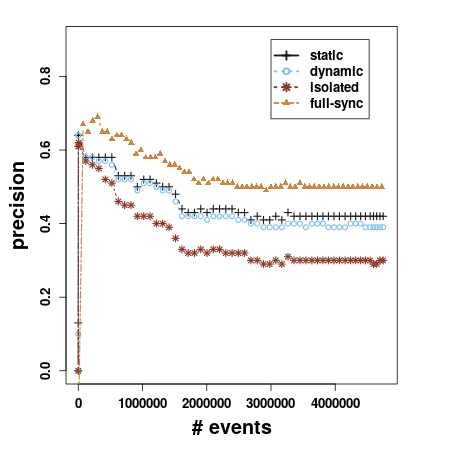
\includegraphics[width=.8\textwidth,height=.7\linewidth]{figures/precision_p1.png}
		.
	\end{center}
	
\end{frame}

\begin{frame}
	
	\frametitle{Empirical evaluation }
	\framesubtitle{Precision scores with respect to the number of input events over time for $\mathcal{P}_1$}
	
	
\end{frame}




\begin{frame}
	
	\frametitle{Empirical evaluation }
	\framesubtitle{Average spread value for $\mathcal{P}_1$}
	
	\begin{center}
		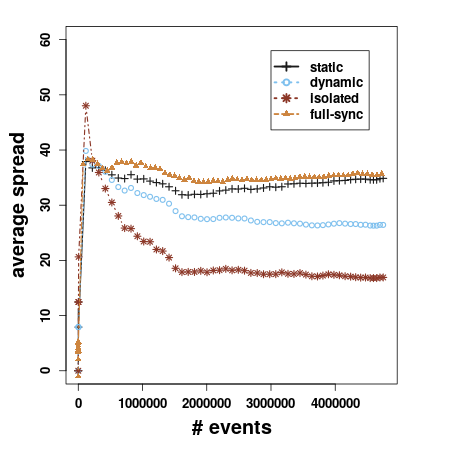
\includegraphics[width=.8\textwidth,height=.7\linewidth]{figures/spread_p1.png}
		.
	\end{center}
	
\end{frame}

\begin{frame}
	
	\frametitle{Empirical evaluation }
	\framesubtitle{Average spread value for $\mathcal{P}_1$}
	

	
\end{frame}




\begin{frame}
	
	\frametitle{Empirical evaluation }
	\framesubtitle{Commutative communication with respect to the number of input events over time for $\mathcal{P}_1$}
	
	\begin{center}
		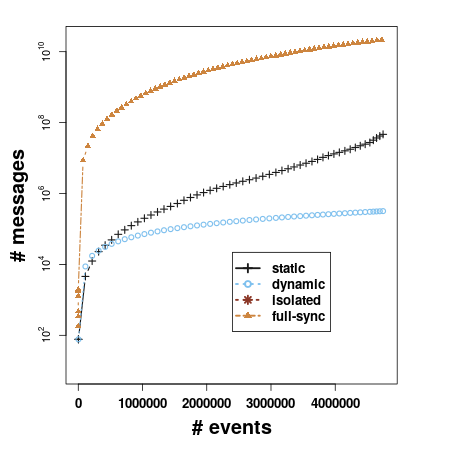
\includegraphics[width=.8\textwidth,height=.7\linewidth]{figures/messages_p1.png}
		.
	\end{center}
	
\end{frame}

\begin{frame}
	
	\frametitle{Empirical evaluation }
	\framesubtitle{Commutative communication with respect to the number of input events over time for $\mathcal{P}_1$}
	
	
	
\end{frame}



\begin{frame}
	
	\frametitle{Empirical evaluation }
	\framesubtitle{Precision scores of $\mathcal{P}_2$  for \textit{PLEASURE CRAFT} vessels}
	
	\begin{center}
		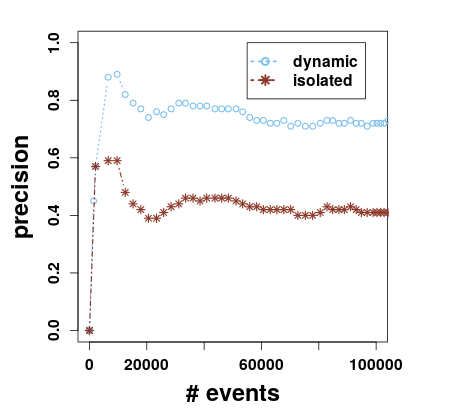
\includegraphics[width=.8\textwidth,height=.7\linewidth]{figures/precision_p2.png}
		.
	\end{center}
	
\end{frame}

\begin{frame}
	
	\frametitle{Empirical evaluation }
	\framesubtitle{Precision scores of $\mathcal{P}_2$  for \textit{PLEASURE CRAFT} vessels}
	

	
\end{frame}
